\documentclass[11pt]{article}
\usepackage[margin=1in]{geometry}
\usepackage{amsmath,amssymb,amsthm}
\usepackage{graphicx}
\usepackage{hyperref}

\newtheorem{theorem}{Theorem}
\newtheorem{corollary}{Corollary}
\newtheorem{lemma}{Lemma}
\newcommand{\C}{\mathbb C}

\title{Linear dependence on the number of simultaneous Riesz selectors}
\author{Full answer to the open problem after Corollary 4.8 of arXiv:2405.18235}
\date{11 August 2026}

\begin{document}
\maketitle

\noindent\textbf{Status.}
\texttt{candidate\_full\_solution\_likely\_valid\_needs\_human\_review}.

\begin{abstract}
Bownik proves that blocks of size
\(O(m^2B/\varepsilon^2)\) suffice for a simultaneous Riesz selector from
\(m\) unit-norm Bessel families of common bound \(B\), and asks whether the
quadratic dependence on \(m\) is optimal. We prove that
\(16mB^2/\varepsilon^2\) suffices. The proof applies the paper's simultaneous
Bessel-selector theorem once to the normalized families and all their
Naimark complements. A cyclic construction gives a matching linear lower
bound for fixed \(B>1+\varepsilon\). Thus the answer is no, and for example at
\(B=2\) the optimal dependence on \(m\) is \(\Theta(m)\).
\end{abstract}

\section{Source problem and proof intuition}

For each \(j\in[m]\), let \((u_i^{(j)})_{i\in I}\) be a unit-norm Bessel
sequence of bound \(B>1\), possibly in a different Hilbert space. Given
pairwise disjoint blocks \((J_k)_{k\in K}\), a selector is a set
\(J\subset\bigcup_kJ_k\) with \(|J\cap J_k|=1\) for every \(k\).

Corollary 4.8 of \cite{source} obtains one selector for which all \(m\)
subfamilies have Riesz bounds \(1-\varepsilon,1+\varepsilon\), provided
\[
 |J_k|\ge C\frac{m^2B}{\varepsilon^2}.
\]
The source then asks whether the quadratic \(m\)-dependence is asymptotically
optimal; see Figure~\ref{fig:source}.

The direct idea is to normalize each family to Bessel bound one and add its
Naimark complement. An upper Bessel estimate on the normalized original gives
the desired upper Riesz bound. The same estimate on its complement gives the
desired lower Riesz bound. Crucially, the squared-norm parameters of each
original/complement pair add to one. Across \(m\) pairs, the simultaneous
selector error therefore depends on \(m\), not \(m^2\).

\section{Two source ingredients}

We isolate the exact consequences of Corollary 3.4 and Lemma 4.3 of
\cite{source}.

\begin{lemma}[Simultaneous Bessel selector]\label{lem:selector}
For \(\ell\) in a finite or countable set \(L\), let
\((w_i^{(\ell)})_{i\in I}\) be Bessel with bound one and suppose
\(\|w_i^{(\ell)}\|^2\le d_\ell\), where \(\sum_{\ell\in L}d_\ell<\infty\).
If \(|J_k|\ge r\) for every selector block, there is a selector \(J\) such
that every \((w_i^{(\ell)})_{i\in J}\) has Bessel bound at most
\[
 d_\ell+\frac1r+2\sqrt{\frac{\sum_{q\in L}d_q}{r}}.
\]
\end{lemma}

\begin{lemma}[Naimark-complement criterion]\label{lem:naimark}
If \((a_i)_{i\in I}\) is Bessel with bound one and
\(\|a_i\|^2=\eta\in(0,1)\), there is a Bessel-one family
\((v_i)_{i\in I}\) with \(\|v_i\|^2=1-\eta\) such that, for every
\(J\subset I\),
\[
 (a_i)_{i\in J}\text{ has lower Riesz bound }\delta
 \quad\Longleftrightarrow\quad
 (v_i)_{i\in J}\text{ has Bessel bound }1-\delta.
\]
\end{lemma}

\section{Linear upper bound}

\begin{theorem}[Linear simultaneous selector]\label{thm:upper}
Let \(m\ge1\), \(B>1\), and \(0<\varepsilon<1\). Suppose that for every
\(j\in[m]\), \((u_i^{(j)})_{i\in I}\) is a unit-norm Bessel sequence of
bound \(B\). If the pairwise disjoint selector blocks satisfy
\[
 |J_k|\ge
 R:=\left\lceil\frac{16mB^2}{\varepsilon^2}\right\rceil,
 \qquad k\in K,
\]
then there is a selector \(J\) such that every
\((u_i^{(j)})_{i\in J}\) is a Riesz sequence with bounds
\(1-\varepsilon\) and \(1+\varepsilon\).
\end{theorem}

\begin{proof}
Put \(\eta=B^{-1}\) and
\(a_i^{(j)}=B^{-1/2}u_i^{(j)}\). Each \(a^{(j)}\) is Bessel with bound one
and \(\|a_i^{(j)}\|^2=\eta\). Lemma~\ref{lem:naimark} supplies a complement
family \(v^{(j)}\) with squared norms \(1-\eta\).

Apply Lemma~\ref{lem:selector} once to all \(2m\) families
\[
 a^{(1)},\ldots,a^{(m)},v^{(1)},\ldots,v^{(m)}.
\]
Their norm parameters sum to
\[
 m\eta+m(1-\eta)=m.
\]
Hence one selector \(J\) simultaneously gives Bessel bounds
\[
 \eta+E_R\quad\text{for every }a^{(j)}|_J,
 \qquad
 1-\eta+E_R\quad\text{for every }v^{(j)}|_J,
\]
where \(E_R=R^{-1}+2\sqrt{m/R}\). The definition of \(R\) gives
\[
 2\sqrt{m/R}\le\frac{\varepsilon}{2B},
 \qquad
 \frac1R\le\frac{\varepsilon}{2B},
\]
the second inequality using \(m\ge1\), \(B>1\), and
\(0<\varepsilon<1\). Thus \(E_R\le\eta\varepsilon\).

The first Bessel estimate is the upper Riesz bound
\(\eta(1+\varepsilon)\) for \(a^{(j)}|_J\). The complement estimate is
\[
 1-\eta+\eta\varepsilon=1-\eta(1-\varepsilon),
\]
so Lemma~\ref{lem:naimark} gives lower Riesz bound
\(\eta(1-\varepsilon)\) for \(a^{(j)}|_J\). Scaling by \(B^{1/2}\)
multiplies both bounds by \(B=\eta^{-1}\), proving the claim.
\end{proof}

For fixed \(B\) and \(\varepsilon\), Theorem~\ref{thm:upper} is linear in
\(m\), already answering the source question negatively. Combined with the
source estimate, it also gives the joint sufficient bound
\[
 O\!\left(\varepsilon^{-2}\min\{mB^2,m^2B\}\right).
\]

\section{The linear exponent is sharp}

\begin{theorem}[Cyclic lower bound]\label{thm:lower}
Fix \(0<\varepsilon<1\) and \(B>1+\varepsilon\). For every \(m\ge1\) and
every \(1\le r\le m\), there are \(m\) unit-norm Bessel families of bound at
most \(B\) and two selector blocks of size \(r\) for which no simultaneous
selector has Riesz bounds \(1-\varepsilon,1+\varepsilon\).
\end{theorem}

\begin{proof}
Choose \(\alpha\) with
\(\varepsilon<\alpha\le\min\{1,B-1\}\). Let
\((e_p)_{p\in\mathbb Z/r\mathbb Z}\) and
\((f_q)_{q\in\mathbb Z/r\mathbb Z}\) be orthonormal and mutually
orthogonal. Use two blocks
\[
 J_0=\{x_p:p\in\mathbb Z/r\mathbb Z\},\qquad
 J_1=\{y_q:q\in\mathbb Z/r\mathbb Z\}.
\]
For \(j\in\mathbb Z/r\mathbb Z\), define
\[
 u_{x_p}^{(j)}=e_p,
 \qquad
 u_{y_q}^{(j)}=\alpha e_{q+j}+\sqrt{1-\alpha^2}\,f_q.
\]
If \(m>r\), repeat any of these families. For fixed \(j\), both displayed
subfamilies are orthonormal, and their cross-Gram matrix is \(\alpha\) times
a permutation matrix. The full Gram matrix therefore has eigenvalues
\(1-\alpha\) and \(1+\alpha\); the family is unit norm and has Bessel bound
\(1+\alpha\le B\).

Any selector is a pair \(\{x_p,y_q\}\). In the family with
\(j=p-q\pmod r\), its two vectors have inner product \(\alpha\), so their
Gram eigenvalues are \(1-\alpha\) and \(1+\alpha\). Since
\(\alpha>\varepsilon\), this selector fails the requested bounds.
\end{proof}

\begin{corollary}[Exact exponent of \(m\)]
For every fixed \(0<\varepsilon<1\) and \(B>1+\varepsilon\), the optimal
universal block size grows as \(\Theta(m)\). In particular this holds for
\(B=2\).
\end{corollary}

\paragraph{Verification and novelty.}
An exact verifier checked 4,050 scalar instances of the upper-bound constants
and all 22,140 cyclic selector pairs through size 40. Four run indexes and
bounded exact-title, exact-question, simultaneous-selector, and Naimark-
complement searches found no prior resolution. Because the proof is a short
combination of two results in \cite{source}, expert novelty review is advised.

\paragraph{Limitation.}
The asymptotic-\(m\) problem is fully answered. The optimal joint dependence
on \(m,B,\varepsilon\) is not determined: the new proof pays \(B^2\), while
the source's proof pays \(m^2B\).

\begin{thebibliography}{9}
\bibitem{source}
M. Bownik,
\emph{Selector form of Weaver's conjecture, Feichtinger's conjecture, and
frame sparsification}, arXiv:2405.18235 (2024).
\end{thebibliography}

\begin{figure}[ht]
\centering
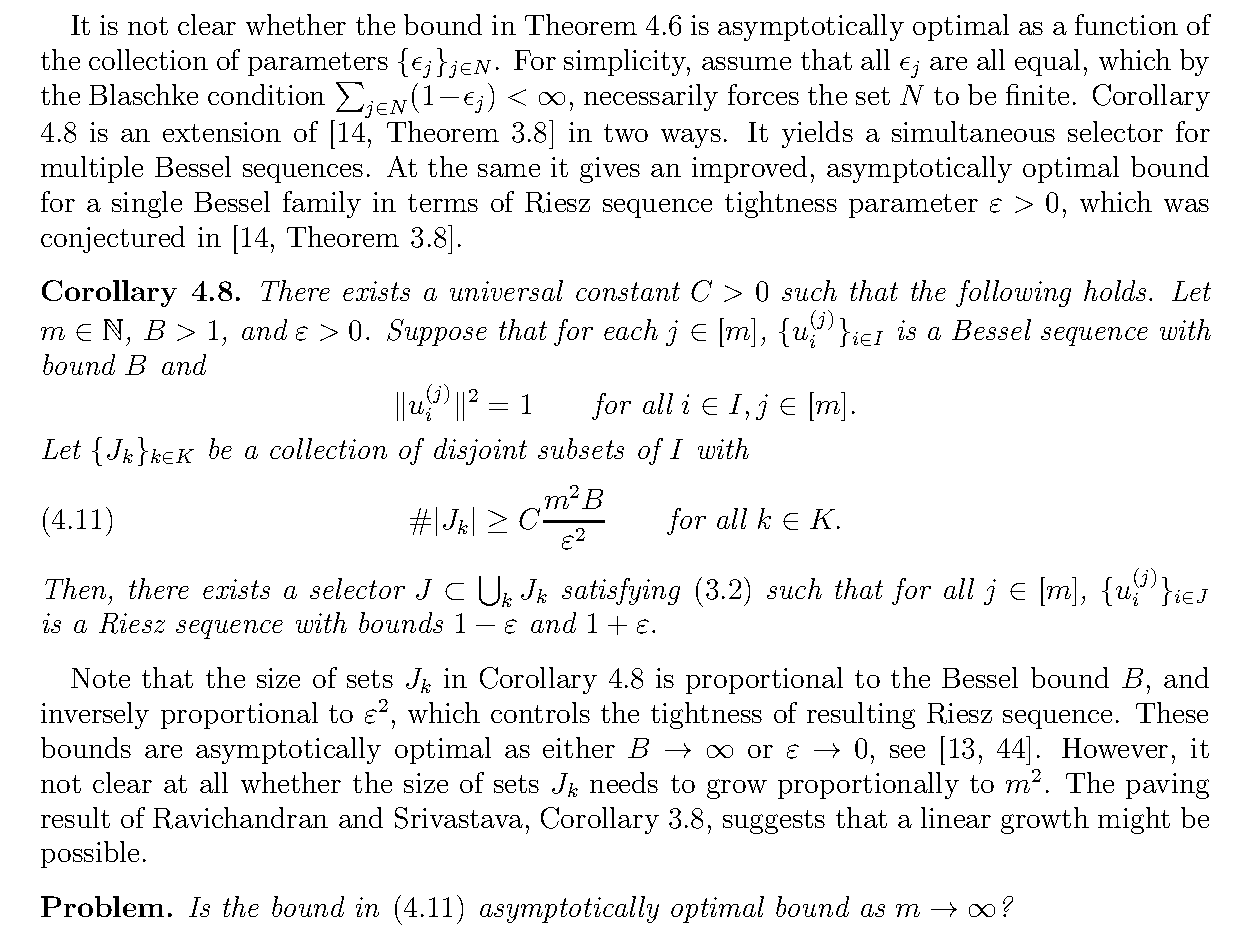
\includegraphics[width=\textwidth]{figures/source_problem_crop.png}
\caption{Source page 26: Corollary 4.8 and the asymptotic-\(m\) problem.}
\label{fig:source}
\end{figure}

\end{document}

